\chapter{Kulit Elektron dan Tabel Periodik}\label{ch:g10:electron-shells}

Neon berpendar merah jingga pada papan reklame; natrium, \omterm{def:g9:periodic-table-first-look:metal}{logam} yang
lunak, \omterm{def:g4:what-a-fire-needs:burning}{terbakar} di dalam air; klorin adalah gas kuning kehijauan yang
menyesakkan napas. Padahal \omterm{def:g7:atoms-and-molecules:atom}{atom-atomnya} hanya berbeda satu atau dua
\omterm{def:g9:inside-the-atom:proton}{proton}: neon memiliki 10, natrium 11, klorin 17. Mengapa unsur-unsur
yang bertetangga dalam \omterm{def:g9:periodic-table-first-look:periodic-table}{tabel periodik} berperilaku begitu berbeda,
sedangkan natrium dan kalium, yang \omterm{def:g9:inside-the-atom:atomic-number}{nomor atomnya} berjauhan, berperilaku
begitu mirip? Jawabannya terletak pada cara \omterm{def:g9:inside-the-atom:nucleus}{elektron-elektron} sebuah
\omterm{def:g7:atoms-and-molecules:atom}{atom} tersusun.

\begin{recall}
Sebuah \omterm{def:g7:atoms-and-molecules:atom}{atom} memiliki $Z$ \omterm{def:g9:inside-the-atom:proton}{proton} di dalam intinya dan, dalam keadaan
netral, $Z$ \omterm{def:g9:inside-the-atom:nucleus}{elektron} di sekelilingnya (\cref{ch:g9:inside-the-atom}).
\omterm{def:g9:periodic-table-first-look:periodic-table}{Tabel periodik} mengurutkan unsur-unsur menurut $Z$ dalam periode (baris)
dan \omterm{def:g9:periodic-table-first-look:period}{golongan} (kolom); unsur-unsur segolongan berperilaku sama
(\cref{ch:g9:periodic-table-first-look}). \omterm{def:g7:atoms-and-molecules:atom}{Atom} menerima atau melepaskan
\omterm{def:g9:inside-the-atom:nucleus}{elektron} untuk menjadi \omterm{def:g9:ions:ion}{ion} (\cref{ch:g9:ions}).
\end{recall}

\section{Konfigurasi elektron}

\begin{definition}[Kulit, subkulit, dan konfigurasi elektron]\label{def:g10:electron-shells:configuration}
\omterm{def:g9:inside-the-atom:nucleus}{Elektron-elektron} sebuah \omterm{def:g7:atoms-and-molecules:atom}{atom} tersusun dalam
\emph{kulit elektron}\index{kulit elektron}, yang diberi nomor
$n = 1, 2, 3, \ldots$ dari inti ke arah luar; makin besar $n$, makin
jauh dari inti dan makin lemah \omterm{def:g9:inside-the-atom:nucleus}{elektron-elektronnya} terikat. Setiap kulit
terbagi menjadi \emph{subkulit}\index{subkulit} yang dinamai dengan
sebuah huruf: kulit 1 memiliki subkulit s (1s), kulit 2 subkulit s dan
p (2s, 2p), kulit 3 memiliki 3s dan 3p (dan 3d, yang akan kita temui
kemudian). Subkulit s menampung paling banyak 2 \omterm{def:g9:inside-the-atom:nucleus}{elektron}, subkulit p
paling banyak 6. Yang disebut
\emph{konfigurasi elektron}\index{konfigurasi elektron} sebuah \omterm{def:g7:atoms-and-molecules:atom}{atom}
adalah daftar subkulit yang terisi beserta banyaknya \omterm{def:g9:inside-the-atom:nucleus}{elektron} di
dalamnya sebagai pangkat: $1\mathrm{s}^2\,2\mathrm{s}^2\,2\mathrm{p}^4$
untuk oksigen.
\end{definition}

\begin{method}[Menuliskan konfigurasi elektron, sampai $Z = 20$]\label{met:g10:electron-shells:write}
\begin{enumerate}
  \item Hitung \omterm{def:g9:inside-the-atom:nucleus}{elektronnya}: $Z$ untuk \omterm{def:g7:atoms-and-molecules:atom}{atom} netral.
  \item Isilah \omterm{def:g10:electron-shells:configuration}{subkulit-subkulit} dengan urutan ini, masing-masing sampai
        penuh sebelum memulai \omterm{def:g10:electron-shells:configuration}{subkulit} berikutnya:
        \[
          1\mathrm{s} \to 2\mathrm{s} \to 2\mathrm{p} \to 3\mathrm{s} \to
          3\mathrm{p} \to 4\mathrm{s}.
        \]
  \item Periksalah bahwa jumlah pangkatnya sama dengan banyaknya \omterm{def:g9:inside-the-atom:nucleus}{elektron}.
\end{enumerate}
Natrium, $Z = 11$: $1\mathrm{s}^2\,2\mathrm{s}^2\,2\mathrm{p}^6\,3\mathrm{s}^1$.
Klorin, $Z = 17$: $1\mathrm{s}^2\,2\mathrm{s}^2\,2\mathrm{p}^6\,3\mathrm{s}^2\,3\mathrm{p}^5$.
Kalsium, $Z = 20$: $1\mathrm{s}^2\,2\mathrm{s}^2\,2\mathrm{p}^6\,3\mathrm{s}^2\,3\mathrm{p}^6\,4\mathrm{s}^2$.
\end{method}

\begin{omfigure}
\begin{tikzpicture}[font=\small, y=0.95cm]
  \draw[->, black!60] (-0.4,0) -- (-0.4,5.4) node[above, align=center, font=\footnotesize]
    {makin jauh\\ dari inti};
  \foreach \y/\lab/\n/\x in {0.3/1s/2/0.5, 1.3/2s/2/0.5, 1.9/2p/6/2.4, 3.0/3s/2/0.5,
      3.6/3p/6/2.4, 4.4/4s/2/0.5} {
    \foreach \k in {1,...,\n} \draw[omDef, fill=omDef!10] (\x+0.42*\k-0.42,\y) rectangle ++(0.36,0.36);
    \node[anchor=east] at (\x-0.05,\y+0.18) {\lab};
  }
  \node[anchor=west, font=\footnotesize] at (5.3,0.48) {kulit 1: paling banyak 2 elektron};
  \node[anchor=west, font=\footnotesize] at (5.3,1.7) {kulit 2: $2 + 6 = 8$};
  \node[anchor=west, font=\footnotesize] at (5.3,3.4) {kulit 3: $2 + 6 = 8$ (sampai $Z = 18$)};
  \node[anchor=west, font=\footnotesize] at (5.3,4.58) {4s terisi sebelum 3d};
\end{tikzpicture}

{\small Urutan pengisian, sampai $Z = 20$. Setiap kotak kecil adalah
tempat bagi satu \omterm{def:g9:inside-the-atom:nucleus}{elektron}: \omterm{def:g10:electron-shells:configuration}{subkulit} s memiliki 2 tempat, \omterm{def:g10:electron-shells:configuration}{subkulit} p 6.}
\end{omfigure}

\section{Elektron valensi}

\begin{definition}[Elektron valensi dan elektron teras]\label{def:g10:electron-shells:valence}
\omterm{def:g9:inside-the-atom:nucleus}{Elektron-elektron} pada \omterm{def:g10:electron-shells:configuration}{kulit terluar} yang terisi (kulit dengan $n$
terbesar) disebut \emph{elektron valensi}\index{elektron valensi};
\omterm{def:g9:inside-the-atom:nucleus}{elektron-elektron} lainnya disebut \emph{elektron teras}\index{elektron teras}.
Hanya \omterm{def:g9:inside-the-atom:nucleus}{elektron} valensi yang ikut serta dalam \omterm{def:g7:chemical-reactions:reaction}{reaksi kimia}.
\end{definition}

\begin{example}[Menghitung elektron valensi]\label{ex:g10:electron-shells:count}
Oksigen, $1\mathrm{s}^2\,2\mathrm{s}^2\,2\mathrm{p}^4$: \omterm{def:g10:electron-shells:configuration}{kulit terluar} $n =
2$, $2 + 4 = 6$ \omterm{def:g10:electron-shells:valence}{elektron valensi}. Natrium, $\ldots 3\mathrm{s}^1$: 1
\omterm{def:g10:electron-shells:valence}{elektron valensi}. Klorin, $\ldots 3\mathrm{s}^2\,3\mathrm{p}^5$: 7.
Neon, $1\mathrm{s}^2\,2\mathrm{s}^2\,2\mathrm{p}^6$: 8, kulit yang penuh.
\end{example}

\section{Tabel periodik disusun ulang dari konfigurasi}

\begin{proposition}[Periode dan golongan dari konfigurasi]\label{prop:g10:electron-shells:table}
Untuk unsur-unsur sampai $Z = 20$:
\begin{itemize}
  \item periode sebuah unsur adalah nomor $n$ \omterm{def:g10:electron-shells:configuration}{kulit terluarnya};
  \item unsur-unsur dalam \omterm{def:g9:periodic-table-first-look:period}{golongan} yang sama memiliki banyak \omterm{def:g10:electron-shells:valence}{elektron
        valensi} yang sama --- satu di \omterm{def:g9:periodic-table-first-look:period}{golongan} 1, dua di \omterm{def:g9:periodic-table-first-look:period}{golongan} 2, tiga
        sampai delapan di \omterm{def:g9:periodic-table-first-look:period}{golongan} 13 sampai 18 (helium, dengan 2, adalah
        pengecualian).
\end{itemize}
Dua kolom paling kiri, tempat \omterm{def:g9:inside-the-atom:nucleus}{elektron-elektron} terakhir masuk ke
\omterm{def:g10:electron-shells:configuration}{subkulit} s, membentuk blok s; \omterm{def:g9:periodic-table-first-look:period}{golongan} 13 sampai 18 membentuk blok p.
\end{proposition}

\begin{omfigure}
\omperiodictable[upto=20, f block=false, cell=0.86cm, colour=blocks, legend=true,
  values={H/1,He/2,Li/2.1,Be/2.2,B/2.3,C/2.4,N/2.5,O/2.6,F/2.7,Ne/2.8,
    Na/2.8.1,Mg/2.8.2,Al/2.8.3,Si/2.8.4,P/2.8.5,S/2.8.6,Cl/2.8.7,Ar/2.8.8,
    K/2.8.8.1,Ca/2.8.8.2}]

{\small Dua puluh unsur pertama, dengan banyaknya \omterm{def:g9:inside-the-atom:nucleus}{elektron} di setiap
kulit di bawah lambangnya ($2.8.1$ untuk natrium: 2 di \omterm{def:g10:electron-shells:configuration}{kulit 1}, 8 di
\omterm{def:g10:electron-shells:configuration}{kulit 2}, 1 di \omterm{def:g10:electron-shells:configuration}{kulit 3}). Warnanya menandai blok s dan blok p.}
\end{omfigure}

\section{Keluarga unsur}

\begin{definition}[Keluarga kimia]\label{def:g10:electron-shells:family}
Sebuah \emph{keluarga kimia}\index{keluarga kimia} adalah \omterm{def:g9:periodic-table-first-look:period}{golongan} dalam
\omterm{def:g9:periodic-table-first-look:periodic-table}{tabel periodik} yang unsur-unsurnya memiliki sifat-sifat kimia utama yang
sama. Tiga keluarga diberi nama: \emph{logam alkali}\index{logam alkali}
(\omterm{def:g9:periodic-table-first-look:period}{golongan} 1 kecuali hidrogen: litium, natrium, kalium\dots), \omterm{def:g9:periodic-table-first-look:metal}{logam} lunak
yang bereaksi kuat dengan air; \emph{halogen}\index{halogen} (\omterm{def:g9:periodic-table-first-look:period}{golongan}
17: fluorin, klorin, bromin, iodin), \omterm{def:g9:periodic-table-first-look:metal}{nonlogam} berwarna yang reaktif; dan
\emph{gas mulia}\index{gas mulia} (\omterm{def:g9:periodic-table-first-look:period}{golongan} 18: helium, neon,
argon\dots), yang hampir tidak bereaksi dengan apa pun.
\end{definition}

\begin{proposition}[Mengapa sebuah keluarga berperilaku sama]\label{prop:g10:electron-shells:why}
Unsur-unsur sebuah keluarga memiliki banyak \omterm{def:g10:electron-shells:valence}{elektron valensi} yang sama,
dan kimia adalah urusan \omterm{def:g10:electron-shells:valence}{elektron valensi}: litium, natrium, dan kalium
semuanya memiliki satu, \omterm{def:g10:electron-shells:family}{halogen} tujuh, \omterm{def:g10:electron-shells:family}{gas mulia} \omterm{def:g10:electron-shells:configuration}{kulit terluar} yang
penuh.
\end{proposition}

\begin{omfigure}
\omperiodictable[colour=families, legend=true, cell=0.86cm, f block=false]

{\small Keluarga-keluarga dalam \omterm{def:g9:periodic-table-first-look:periodic-table}{tabel periodik}: \omterm{def:g10:electron-shells:family}{logam alkali}, \omterm{def:g10:electron-shells:family}{logam
alkali} tanah (\omterm{def:g9:periodic-table-first-look:period}{golongan} 2), \omterm{def:g10:electron-shells:family}{halogen}, dan \omterm{def:g10:electron-shells:family}{gas mulia}.}
\end{omfigure}

\begin{omfigure}
\begin{minipage}[b]{0.48\linewidth}\centering
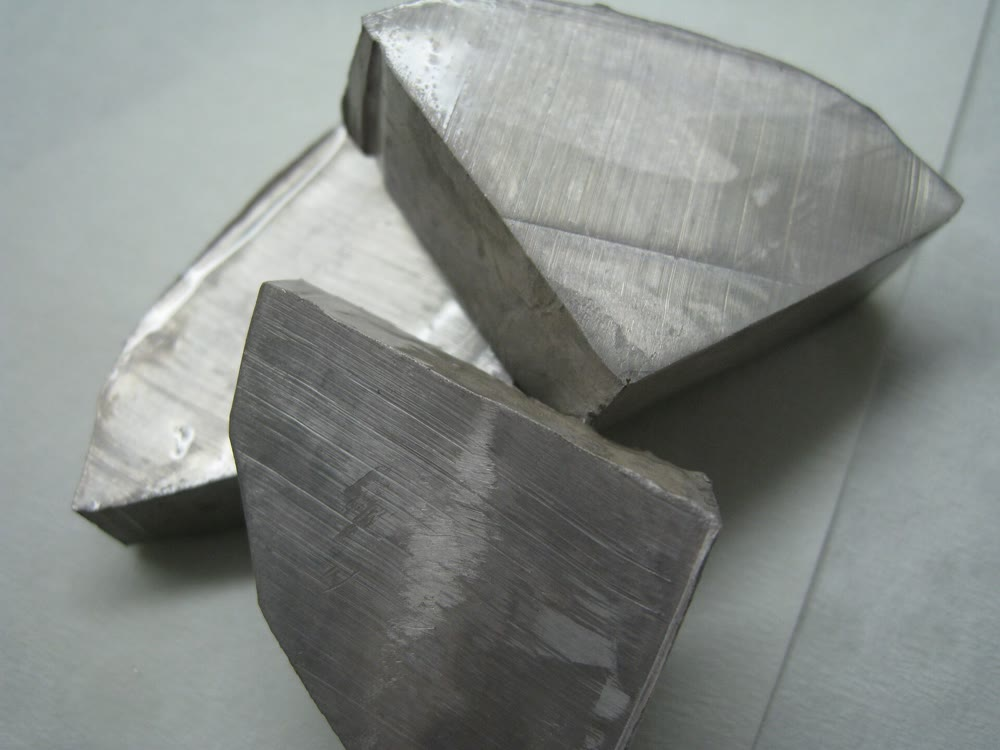
\includegraphics[width=\linewidth,height=4.4cm,keepaspectratio]{images/book1/sodium.jpg}

{\small Natrium, sebuah \omterm{def:g10:electron-shells:family}{logam alkali}, dipotong dengan pisau: lunak dan
keperakan ketika baru dipotong, natrium langsung kusam di \omterm{def:g4:air-a-mixture-of-gases:air}{udara}. Foto:
Dnn87, CC\ BY-SA\ 3.0.}
\end{minipage}\hfill
\begin{minipage}[b]{0.48\linewidth}\centering
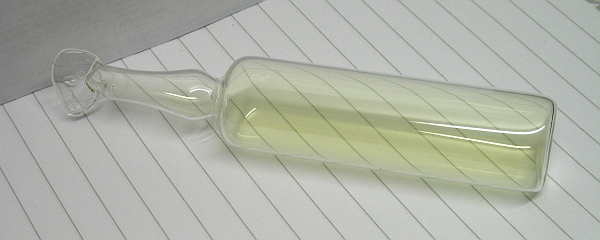
\includegraphics[width=\linewidth,height=4.4cm,keepaspectratio]{images/book1/chlorine-ampoule.jpg}

{\small Klorin, sebuah \omterm{def:g10:electron-shells:family}{halogen}: gas kuning kehijauan, di sini tersegel
di dalam ampul kaca. Foto: W.~Oelen, CC\ BY-SA\ 3.0.}
\end{minipage}
\end{omfigure}

\begin{inthelab}[Natrium dalam air]
Di balik layar pelindung, guru menjatuhkan sepotong natrium sebesar
sebutir beras ke dalam baskom besar berisi air. Natrium itu terapung,
meleleh menjadi bola mengilap, dan berlari ke sana kemari sambil
berdesis sampai habis; gas yang dilepaskan adalah hidrogen, dan air yang
tersisa bersifat basa.
\end{inthelab}

\begin{safety}{\ghs[0.75cm]{GHS02}\ghs[0.75cm]{GHS05}\quad\ghs[0.75cm]{GHS03}\ghs[0.75cm]{GHS06}}
% ledger: ghs:Na, ghs:Cl2
Natrium: melepaskan hidrogen yang mudah menyala jika bersentuhan dengan
air (GHS02), menyebabkan luka bakar parah (GHS05). Klorin: gas
pengoksidasi (GHS03), beracun jika terhirup (GHS06), juga iritan dan
sangat beracun bagi kehidupan akuatik. Keduanya hanya ditangani oleh
guru.
\end{safety}

\section{Ion yang stabil dan aturan gas mulia}

\begin{definition}[Aturan duplet dan oktet]\label{def:g10:electron-shells:octet}
\omterm{def:g10:electron-shells:family}{Gas mulia}, dengan \omterm{def:g10:electron-shells:configuration}{kulit terluar} yang penuh, hampir tidak bereaksi:
konfigurasinya sangat stabil. Ketika \omterm{def:g7:atoms-and-molecules:atom}{atom-atom} unsur pertama membentuk
\omterm{def:g9:ions:ion}{ion}, \omterm{def:g7:atoms-and-molecules:atom}{atom-atom} itu menerima atau melepaskan \omterm{def:g9:inside-the-atom:nucleus}{elektron} sehingga mencapai
konfigurasi \omterm{def:g10:electron-shells:family}{gas mulia} terdekat: dua \omterm{def:g9:inside-the-atom:nucleus}{elektron} di \omterm{def:g10:electron-shells:configuration}{kulit 1}, seperti helium,
untuk \omterm{def:g7:atoms-and-molecules:atom}{atom-atom} yang paling ringan --- \emph{aturan duplet}\index{aturan duplet}
--- dan delapan \omterm{def:g9:inside-the-atom:nucleus}{elektron} di \omterm{def:g10:electron-shells:configuration}{kulit terluar}, seperti neon atau argon,
untuk \omterm{def:g7:atoms-and-molecules:atom}{atom-atom} lainnya --- \emph{aturan oktet}\index{aturan oktet}.
\end{definition}

\begin{example}[Ion-ion yang diramalkan aturan itu]\label{ex:g10:electron-shells:ions}
Natrium, $2.8.1$, melepaskan satu-satunya \omterm{def:g10:electron-shells:valence}{elektron valensinya}: \ce{Na+},
$2.8$, seperti neon. Magnesium, $2.8.2$, melepaskan dua: \ce{Mg^{2+}}.
Aluminium, $2.8.3$, melepaskan tiga: \ce{Al^{3+}}. Klorin, $2.8.7$,
menerima satu: \ce{Cl-}, $2.8.8$, seperti argon. Oksigen, $2.6$,
menerima dua: \ce{O^{2-}}. Belerang, $2.8.6$: \ce{S^{2-}}. Litium,
$2.1$, melepaskan satu dan menyisakan $2$, seperti helium: \ce{Li+}.
\end{example}

\begin{omfigure}
\begin{tikzpicture}[font=\small]
  \foreach \x/\nm/\cfg/\col in {0/{Na}/{$1\mathrm{s}^2\,2\mathrm{s}^2\,2\mathrm{p}^6\,3\mathrm{s}^1$}/omDef,
      5.8/{\ce{Na+}}/{$1\mathrm{s}^2\,2\mathrm{s}^2\,2\mathrm{p}^6$}/omProp,
      11.0/{Ne}/{$1\mathrm{s}^2\,2\mathrm{s}^2\,2\mathrm{p}^6$}/gray} {
    \node[draw=\col, fill=\col!6, rounded corners=2pt, align=center, text width=3.4cm]
      at (\x,0) {\textbf{\nm}\\ \cfg};
  }
  \draw[->, thick, omProp] (2.0,0) -- (3.8,0) node[midway, above, font=\footnotesize] {melepas 1 \ce{e-}};
  \node at (8.4,0) {$=$};
  \node[font=\footnotesize, align=center] at (8.4,-0.75) {konfigurasi\\ sama};
\end{tikzpicture}

{\small \omterm{def:g9:ions:ion}{Ion} natrium memiliki konfigurasi neon, \omterm{def:g10:electron-shells:family}{gas mulia} yang terdekat.}
\end{omfigure}

\begin{remark}[Batas-batas aturan itu]\label{rem:g10:electron-shells:limits}
Aturan itu berlaku baik untuk dua puluh unsur pertama dan \omterm{def:g9:ions:ion}{ion-ion}
sederhananya. Banyak unsur, seperti besi (\ce{Fe^{2+}} dan \ce{Fe^{3+}}),
tidak mengikutinya; alasan-alasannya, beserta gambaran yang lebih baik
tentang \omterm{def:g9:inside-the-atom:nucleus}{elektron}, diberikan dalam buku Tahun Pertama universitas.
\end{remark}

\section{Latihan}

\begin{exercise}[$\star$]\label{exo:g10:electron-shells:1}
Tuliskan \omterm{def:g10:electron-shells:configuration}{konfigurasi elektron} karbon ($Z = 6$), nitrogen ($Z = 7$), dan
magnesium ($Z = 12$).
\end{exercise}

\begin{exercise}[$\star$]\label{exo:g10:electron-shells:2}
Berapa \omterm{def:g10:electron-shells:valence}{elektron valensi} yang dimiliki karbon, nitrogen, dan magnesium?
\end{exercise}

\begin{exercise}[$\star$]\label{exo:g10:electron-shells:3}
Pada periode dan \omterm{def:g9:periodic-table-first-look:period}{golongan} berapa unsur yang konfigurasinya
$1\mathrm{s}^2\,2\mathrm{s}^2\,2\mathrm{p}^6\,3\mathrm{s}^2\,3\mathrm{p}^3$?
\end{exercise}

\begin{exercise}[$\star$]\label{exo:g10:electron-shells:4}
Sebutkan ketiga keluarga dalam bab ini dan berikan dua unsur dari
masing-masing.
\end{exercise}

\begin{exercise}[$\star$]\label{exo:g10:electron-shells:5}
Nyatakan \omterm{def:g10:electron-shells:octet}{aturan oktet}.
\end{exercise}

\begin{exercise}[$\star\star$]\label{exo:g10:electron-shells:6}
Dengan aturan \omterm{def:g10:electron-shells:family}{gas mulia}, tentukan \omterm{def:g9:ions:ion}{ion} yang dibentuk kalium ($Z = 19$)
dan fluorin ($Z = 9$), beserta konfigurasinya.
\end{exercise}

\begin{exercise}[$\star\star$]\label{exo:g10:electron-shells:7}
Sebuah unsur memiliki 2 \omterm{def:g9:inside-the-atom:nucleus}{elektron} di \omterm{def:g10:electron-shells:configuration}{kulit ketiganya}, dan \omterm{def:g10:electron-shells:configuration}{kulit ketiga} itu
adalah \omterm{def:g10:electron-shells:configuration}{kulit terluarnya}. Tentukan konfigurasinya, \omterm{def:g9:inside-the-atom:atomic-number}{nomor atomnya}, dan
namanya.
\end{exercise}

\begin{exercise}[$\star\star$]\label{exo:g10:electron-shells:8}
Dengan \omterm{def:g9:ions:ion}{ion-ion} yang stabil, tuliskan rumus \omterm{def:g9:ions:ionic-compound}{senyawa ion} yang dibentuk
magnesium dan klorin, lalu aluminium dan oksigen.
\end{exercise}

\begin{exercise}[$\star\star$]\label{exo:g10:electron-shells:9}
Lihatlah tabel dua puluh unsur pertama. Unsur-unsur apa yang memiliki
banyak \omterm{def:g10:electron-shells:valence}{elektron valensi} yang sama dengan oksigen?
\end{exercise}

\begin{exercise}[$\star\star$]\label{exo:g10:electron-shells:10}
Mengapa neon, tidak seperti natrium dan klorin, tidak membentuk \omterm{def:g9:ions:ion}{ion}
dalam \omterm{def:g7:chemical-reactions:reaction}{reaksi kimia}?
\end{exercise}

\begin{exercise}[$\star\star$]\label{exo:g10:electron-shells:11}
\omterm{def:g9:ions:ion}{Ion} \ce{X^{2+}} memiliki konfigurasi argon. Tentukan $X$.
\end{exercise}

\begin{exercise}[$\star\star\star$]\label{exo:g10:electron-shells:12}
Helium memiliki 2 \omterm{def:g10:electron-shells:valence}{elektron valensi} tetapi berada di \omterm{def:g9:periodic-table-first-look:period}{golongan} 18, bukan
\omterm{def:g9:periodic-table-first-look:period}{golongan} 2. Jelaskan dengan konfigurasinya.
\end{exercise}

\begin{exercise}[$\star\star\star$]\label{exo:g10:electron-shells:13}
Kalium bereaksi dengan air bahkan lebih hebat daripada natrium. Dengan
jarak \omterm{def:g10:electron-shells:valence}{elektron valensinya} dari inti, berikan dugaan mengapa.
\end{exercise}

\begin{exercise}[$\star\star\star$]\label{exo:g10:electron-shells:14}
Tuliskan konfigurasi \ce{S^{2-}}, \ce{Cl-}, \ce{K+}, dan \ce{Ca^{2+}}.
Apa persamaan keempatnya?
\end{exercise}

\begin{exercise}[$\star\star\star$]\label{exo:g10:electron-shells:15}
Sebuah unsur periode 3 membentuk \omterm{def:g9:ions:ion}{ion} \ce{Y^{3-}}. Tentukan \omterm{def:g9:periodic-table-first-look:period}{golongannya},
konfigurasinya, dan namanya.
\end{exercise}

\section{Soal: Rubi, Safir, dan Korundum}

\begin{problem}[{Soal akhir pekan --- elektron di balik sebuah batu
permata: dari dua konfigurasi sampai banyaknya elektron yang berpindah
dalam satu gram}]
\label{pb:g10:electron-shells:1}
Rubi dan safir adalah bentuk permata dari korundum, \omterm{def:g9:ions:ionic-compound}{senyawa ion}
aluminium dan oksigen; sedikit \omterm{def:g9:periodic-table-first-look:metal}{logam} lain memberinya warna. Korundum
cukup keras untuk menggores hampir apa saja, dan serbuk korundum dipakai
untuk memoles lensa. Anggaplah massa sebuah \omterm{def:g9:inside-the-atom:proton}{nukleon} \qty{1.67e-27}{kg};
aluminium-27 memiliki 27 \omterm{def:g9:inside-the-atom:proton}{nukleon}, oksigen-16 memiliki 16.

\medskip
\noindent\textbf{Bagian I --- \omterm{def:g7:atoms-and-molecules:atom}{Atom-atomnya}.}
\begin{enumerate}
  \item Tentukan banyaknya \omterm{def:g9:inside-the-atom:proton}{proton} dan \omterm{def:g9:inside-the-atom:nucleus}{elektron} sebuah \omterm{def:g7:atoms-and-molecules:atom}{atom} aluminium
        ($Z = 13$) dan sebuah \omterm{def:g7:atoms-and-molecules:atom}{atom} oksigen ($Z = 8$).
  \item Tuliskan \omterm{def:g10:electron-shells:configuration}{konfigurasi elektron} keduanya.
  \item Berapa \omterm{def:g10:electron-shells:valence}{elektron valensi} yang dimiliki masing-masing? Pada periode
        dan \omterm{def:g9:periodic-table-first-look:period}{golongan} berapa masing-masing berada?
  \item Apakah aluminium \omterm{def:g9:periodic-table-first-look:metal}{logam} atau \omterm{def:g9:periodic-table-first-look:metal}{nonlogam}? Dan oksigen?
\end{enumerate}

\medskip
\noindent\textbf{Bagian II --- \omterm{def:g9:ions:ion}{Ion-ionnya}.}
\begin{enumerate}[resume]
  \item Dengan \omterm{def:g10:electron-shells:octet}{aturan oktet}, \omterm{def:g9:ions:ion}{ion} apa yang dibentuk aluminium? Tuliskan
        konfigurasinya.
  \item \omterm{def:g9:ions:ion}{Ion} apa yang dibentuk oksigen? Tuliskan konfigurasinya.
  \item \omterm{def:g10:electron-shells:family}{Gas mulia} apa yang memiliki konfigurasi yang sama dengan kedua \omterm{def:g9:ions:ion}{ion}
        itu?
  \item Berapa \omterm{def:g9:inside-the-atom:nucleus}{elektron} yang dilepaskan sebuah \omterm{def:g7:atoms-and-molecules:atom}{atom} aluminium, dan berapa
        yang diterima sebuah \omterm{def:g7:atoms-and-molecules:atom}{atom} oksigen?
\end{enumerate}

\medskip
\noindent\textbf{Bagian III --- Rumusnya.}
\begin{enumerate}[resume]
  \item Tentukan rumus korundum, senyawa netral dari \omterm{def:g9:ions:ion}{ion-ion} ini.
  \item Dalam satu satuan rumus, berapa \omterm{def:g9:inside-the-atom:nucleus}{elektron} yang dilepaskan \omterm{def:g7:atoms-and-molecules:atom}{atom-atom}
        aluminium? Yang diterima \omterm{def:g7:atoms-and-molecules:atom}{atom-atom} oksigen?
  \item Mengapa kedua bilangan itu harus sama?
  \item Sebutir rubi mengandung sedikit \omterm{def:g9:ions:ion}{ion} kromium \ce{Cr^{3+}} yang
        menggantikan sebagian \ce{Al^{3+}}. Mengapa \omterm{def:g9:ions:ion}{ion} \ce{Cr^{3+}} dapat
        menggantikan \omterm{def:g9:ions:ion}{ion} \ce{Al^{3+}} tanpa mengganggu keseimbangan
        muatan?
\end{enumerate}

\medskip
\noindent\textbf{Bagian IV --- Satu gram korundum.}
\begin{enumerate}[resume]
  \item Berapa \omterm{def:g9:inside-the-atom:proton}{nukleon} yang ada dalam satu satuan rumus korundum?
  \item Hitung massa satu satuan rumus (\omterm{def:g9:inside-the-atom:nucleus}{elektron} diabaikan).
  \item Berapa satuan rumus yang ada dalam \qty{1}{g} korundum?
  \item Berapa \omterm{def:g9:ions:ion}{ion} \ce{Al^{3+}} dan \omterm{def:g9:ions:ion}{ion} \ce{O^{2-}} itu?
  \item Mengapa \omterm{def:g9:inside-the-atom:nucleus}{elektron} dapat diabaikan pada soal 14?
  \item Berapa \omterm{def:g9:inside-the-atom:nucleus}{elektron} yang berpindah dari aluminium ke oksigen untuk
        membentuk \qty{1}{g} korundum?
\end{enumerate}
\end{problem}
